\documentclass[14,fleqn]{article}
\usepackage{amsmath}
\usepackage{amssymb}
\usepackage[top=.5 in,left=.5 in,right=.5 in,bottom=.5 in]{geometry}
\usepackage{enumerate}
\usepackage{ mathrsfs }
\usepackage{graphicx}
\usepackage{pgf,tikz}
\usepackage{mathrsfs}
\usepackage{gensymb}
\usepackage{venndiagram}
\usetikzlibrary{arrows}

\pagenumbering{gobble}

\setlength{\parindent}{0 pt}
\setlength{\parskip}{1 ex}

\newcommand{\lcm}{\textnormal{lcm}}
\newcommand{\norm}{\triangleleft}
\newcommand{\bfm}[1]{$\boldsymbol{#1}$}
\newcommand{\Z}{\ensuremath{\mathbb{Z}}}
\newcommand{\R}{\ensuremath{\mathbb{R}}}
\newcommand{\C}{\ensuremath{\mathbb{C}}}
\renewcommand{\wedge}[1]{\ensuremath{\langle #1 \rangle}}
\newcommand{\infsum}[1]{\ensuremath{\sum_{n=#1}^\infty}}
\newcommand{\defn}[1]{\textbf{\underline{#1}}}


\begin{document}
\section{Section 5.2: A Fundamental Principle of Counting}
If $A$ is a set then we will define $n(A)$ or $|A|$ to be the number of elements in $A.$ For example
\[
	|\{1,2,3,4,5\}|=5\quad |\{a,c,e\}|=3 \quad |\emptyset|=0
\]

Many interesting problems can be phrased as finding how many elements are in some set. One of our first questions is ``What is $n(A\cup B)$?''\\
Explore with the worksheet.

A tool for analyzing sets is the Venn-Diagram.\\
\begin{center}
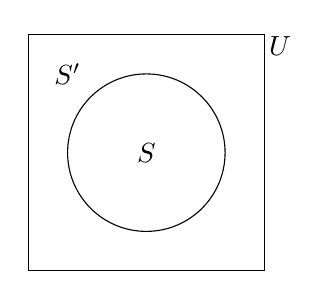
\begin{tikzpicture}[scale=.5]
	\draw[fill=white] (0,0) rectangle (6,6);
	\draw[fill=white] (3,3) circle [radius=2];
	\draw (3,3) node {$S$};
	\draw (1,5) node {$S'$};
	\draw (6.4,5.7) node {$U$};
\end{tikzpicture}
\end{center}

It gives a visual representation of a set $S$ in the universal set $U.$ The complement of a set is represented by the space outside. We can also use them to represent the interaction between sets.
\begin{center}
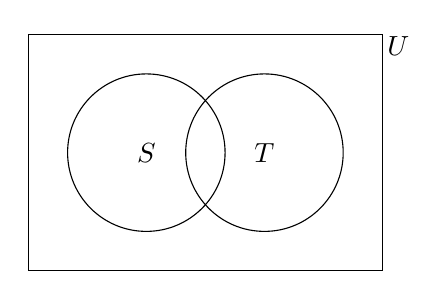
\begin{tikzpicture}[scale=.5]
	\draw[] (0,0) rectangle (9,6);
	\draw[] (3,3) circle [radius=2];
	\draw[] (6,3) circle [radius=2];
	\draw (3,3) node {$S$};
	\draw (6,3) node {$T$};
	\draw (9.4,5.7) node {$U$};
\end{tikzpicture}
\end{center}

For example, suppose we want to visualize $S\cap T'.$ we can first draw the diagrams for $S$ and $T'$ then then see the areas which are shaded in both.
\begin{center}
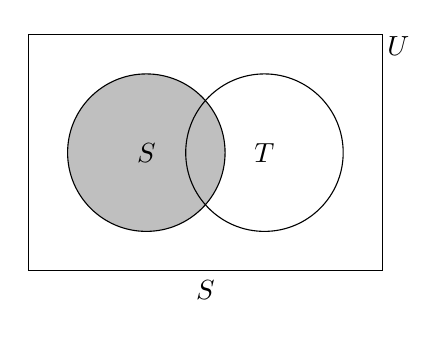
\begin{tikzpicture}[scale=.5]
	\draw[] (0,0) rectangle (9,6);
	\draw[fill=lightgray] (3,3) circle [radius=2];
	\draw[] (6,3) circle [radius=2];
	\draw (3,3) node {$S$};
	\draw (6,3) node {$T$};
	\draw (9.4,5.7) node {$U$};
	\draw (4.5,-0.5) node {$S$};
\end{tikzpicture}
\hspace*{1 in}
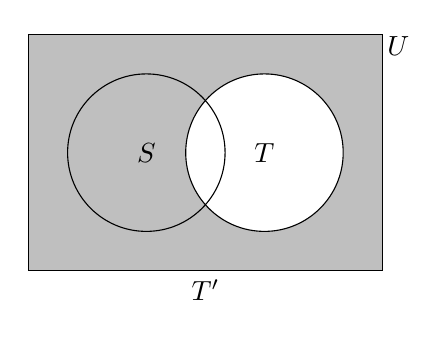
\begin{tikzpicture}[scale=.5]
	\draw[fill=lightgray] (0,0) rectangle (9,6);
	\draw[fill=white] (6,3) circle [radius=2];
	\draw[] (3,3) circle [radius=2];
	\draw (3,3) node {$S$};
	\draw (6,3) node {$T$};
	\draw (9.4,5.7) node {$U$};
	\draw (4.5,-0.5) node {$T'$};
\end{tikzpicture}\\
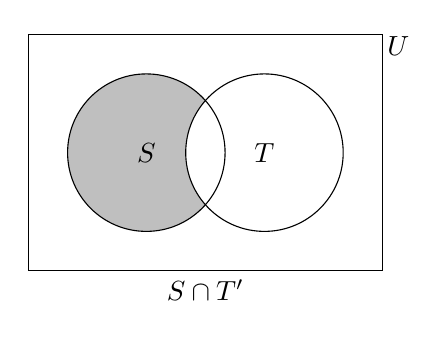
\begin{tikzpicture}[scale=.5]
	\draw[] (0,0) rectangle (9,6);
	\draw[fill=lightgray,draw=none] (3,3) circle [radius=2];
	\draw[fill=white] (6,3) circle [radius=2];
	\draw[] (3,3) circle [radius=2];
	\draw (3,3) node {$S$};
	\draw (6,3) node {$T$};
	\draw (9.4,5.7) node {$U$};
	\draw (4.5,-0.5) node {$S\cap T'$};
\end{tikzpicture}
\end{center}
\pagebreak
If we want to visualize a union, we can do the same thing except we look at the regions shaded in either figure. Let's try to visualize $S\cup T.$
\begin{center}
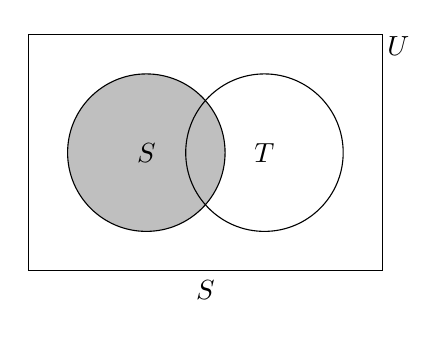
\begin{tikzpicture}[scale=.5]
	\draw[] (0,0) rectangle (9,6);
	\draw[fill=lightgray] (3,3) circle [radius=2];
	\draw[] (6,3) circle [radius=2];
	\draw (3,3) node {$S$};
	\draw (6,3) node {$T$};
	\draw (9.4,5.7) node {$U$};
	\draw (4.5,-0.5) node {$S$};
\end{tikzpicture}
\hspace*{1 in}
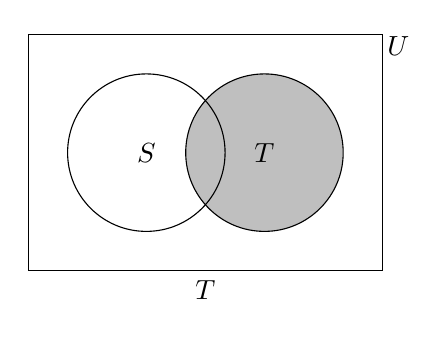
\begin{tikzpicture}[scale=.5]
	\draw[] (0,0) rectangle (9,6);
	\draw[fill=lightgray] (6,3) circle [radius=2];
	\draw[] (3,3) circle [radius=2];
	\draw (3,3) node {$S$};
	\draw (6,3) node {$T$};
	\draw (9.4,5.7) node {$U$};
	\draw (4.5,-0.5) node {$T$};
\end{tikzpicture}\\
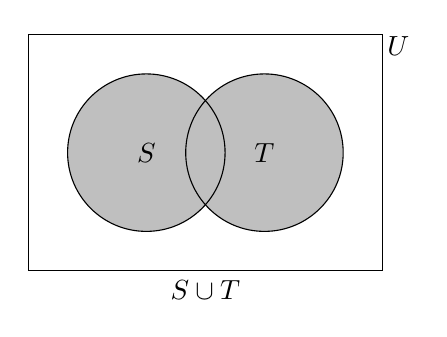
\begin{tikzpicture}[scale=.5]
	\draw[] (0,0) rectangle (9,6);
	\draw[fill=lightgray,draw=none] (3,3) circle [radius=2];
	\draw[fill=lightgray] (6,3) circle [radius=2];
	\draw[] (3,3) circle [radius=2];
	\draw (3,3) node {$S$};
	\draw (6,3) node {$T$};
	\draw (9.4,5.7) node {$U$};
	\draw (4.5,-0.5) node {$S\cup T$};
\end{tikzpicture}
\end{center}

We can also use this to analyze more than 2 sets. We can make a Venn Diagram with 3 sets that looks like\\
\begin{center}
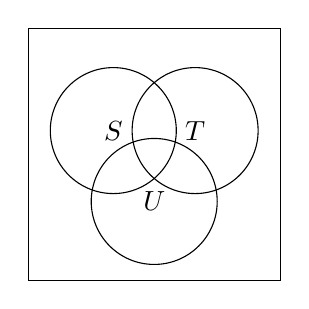
\begin{tikzpicture}[scale=.2]
	\draw (-8,-8) rectangle (8,8);
	\draw (30:3) circle [radius=4];
	\draw (150:3) circle [radius=4];
	\draw (270:3) circle [radius=4];	
	\draw (30:3) node {$T$};
	\draw (150:3) node {$S$};
	\draw (270:3) node {$U$};
\end{tikzpicture}
\end{center}

Let's use one of these to analyze the set $S\cup (T'\cap U).$\\
\begin{venndiagram3sets}[labelA=$S$,labelB=$T$,labelC=$U$]
	\fillA
	\fillOnlyC
\end{venndiagram3sets}\\
We can also use Venn Diagrams to prove some properties about sets. Two of the most useful such relations are known as DeMorgan's laws:
\[
	(S\cap T)'=S'\cup T' \qquad (S\cup T)'=S'\cap T'
\]
We can prove relations by drawing Venn diagrams for both sides and then visually comparing them to check if they are the same. Let's try it with the first relation.\\
First we examine the left hand side of the relation.
\begin{center}
\begin{venndiagram2sets}[labelA=$S$,labelB=$T$]
	\fillACapB
	\setpostvennhook{
		\draw[] (labelAB) ++(0,-2.1) node {\raisebox{0pt}[0pt][0pt]{$S\cap T$}};
	}
\end{venndiagram2sets}
\hspace{1 in}
\begin{venndiagram2sets}[labelA=$S$,labelB=$T$]
	\fillNotA
	\fillNotB
	\setpostvennhook{
		\draw[] (labelAB) ++(0,-2.1) node {\raisebox{0pt}[0pt][0pt]{$(S\cap T)'$}};
	}
\end{venndiagram2sets}\\
Then we look at the right hand side of the relation.\\
\begin{venndiagram2sets}[labelA=$S$,labelB=$T$]
	\fillNotA
	\setpostvennhook{
		\draw[] (labelAB) ++(0,-2.1) node {\raisebox{0pt}[0pt][0pt]{$S'$}};
	}
\end{venndiagram2sets}
\hspace{1 in}
\begin{venndiagram2sets}[labelA=$S$,labelB=$T$]
	\fillNotB
	\setpostvennhook{
		\draw[] (labelAB) ++(0,-2.1) node {\raisebox{0pt}[0pt][0pt]{$T'$}};
	}
\end{venndiagram2sets}\\
\begin{venndiagram2sets}[labelA=$S$,labelB=$T$]
	\fillNotAorNotB
	\setpostvennhook{
		\draw[] (labelAB) ++(0,-2.1) node {\raisebox{0pt}[0pt][0pt]{$S'\cup T'$}};
	}
\end{venndiagram2sets}\\
\end{center}
Since these sets look the same we have verified the first relation. Try the same thing with the other relation.

Now prove the following relation using Venn Diagrams: $(A\cap B)\cup (B\cap C) \cup (A\cap C)\subset A\cup B$



\end{document}
